\documentclass{article}

% Packages
\usepackage[utf8]{inputenc} % UTF-8 input encoding
\usepackage[T1]{fontenc} % Font encoding
\usepackage{amsmath, amssymb} % Math packages
\usepackage{enumitem} % For customizing lists
\usepackage{lipsum} % For generating dummy text
\usepackage{listings}
\usepackage{graphicx}


\lstset{%
  language=bash,
  basicstyle=\fontfamily{pcr}\selectfont,
  commentstyle=\bfseries,
  escapeinside={(*@}{@*)}
}

\newcommand{\comment}[1]{\# here is a comment: #1}
\newcommand\floor[1]{\lfloor#1\rfloor}
\newcommand\ceil[1]{\lceil#1\rceil}

% Title and author information
\title{Algorithms (6470) HW03b}
\author{Alex Darwiche}
\date{\today}

\begin{document}

\maketitle

\section*{Answers}

% Question 1
\subsection*{Q1}
\begin{enumerate}[label=(\alph*)]
    \item Prove the greedy choice property for the fraction knapsack is optimal:
    \item For this proof, we will use contradiction.
    \item The proof begins with the following assumptions:
    \subitem (1) The greedy selection criteria is $max(\frac{v_i}{w_i})$
    \subitem (2) Knowing that, we can assume that there is an item i with with the highest $\frac{v_i}{w_i}$.
    \item For contradiction, we want to prove that an optimal solution exists that doesn't have the max amount of item i as possible.
    \item Assumption: There exists a solution where $V_2 > V_1$ given a lesser amount of item i.
    \item Step 1: Let's subtract $V_2-V_1$
    \subitem (1) With this subtraction, we will be left with: 
    \subitem (2) $V_2-V_1$ = $(y-x)(v_i) + (x)(v_j) - (y)(v_i)$
    \subitem (3) In this equation, y = the weight of item i in the $V_1$ and x = the weight of item j used to replace item i in $V_2$. 
    \subitem (4) Simplify, $V_2-V_1$ = $y*v_i-x*v_i + x*v_j - y*v_i$ = $x*v_j - x*v_i$
    \subitem (5) So, with the assumption that item i has the $max(\frac{v_i}{w_i})$, then $x*v_j - x*v_i < 0$ given they both have the same amount x.
    \subitem (6) So, $V_2-V_1 < 0$ or $V_2 < V_1$. This contradicts are earlier statement, thus proving the greey choice property of the fractional knapsack problem.

\end{enumerate}

% Question 2
\subsection*{Q2}
\begin{enumerate}[label=(\alph*)]
    \item Huffman Encoding:
    \subitem 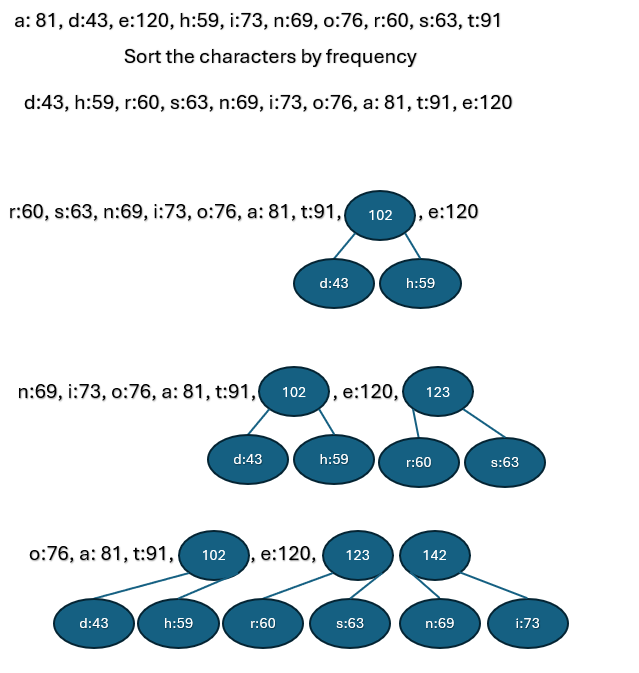
\includegraphics[width=.65\textwidth]{huffman1.png}
    \subitem 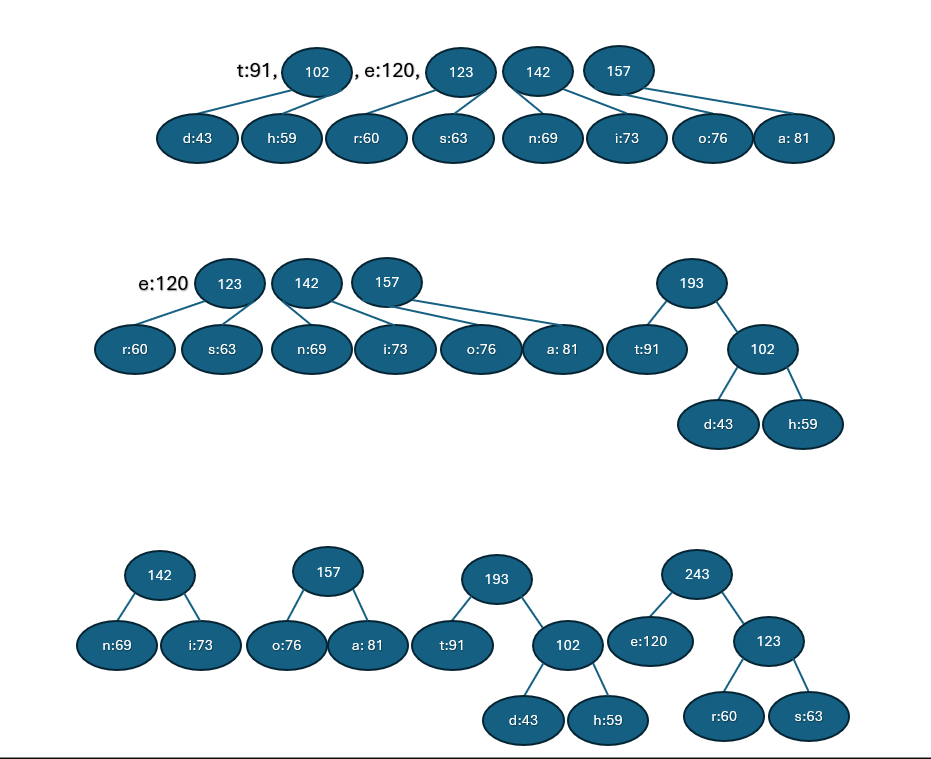
\includegraphics[width=.65\textwidth]{huffman2.png}
    \subitem 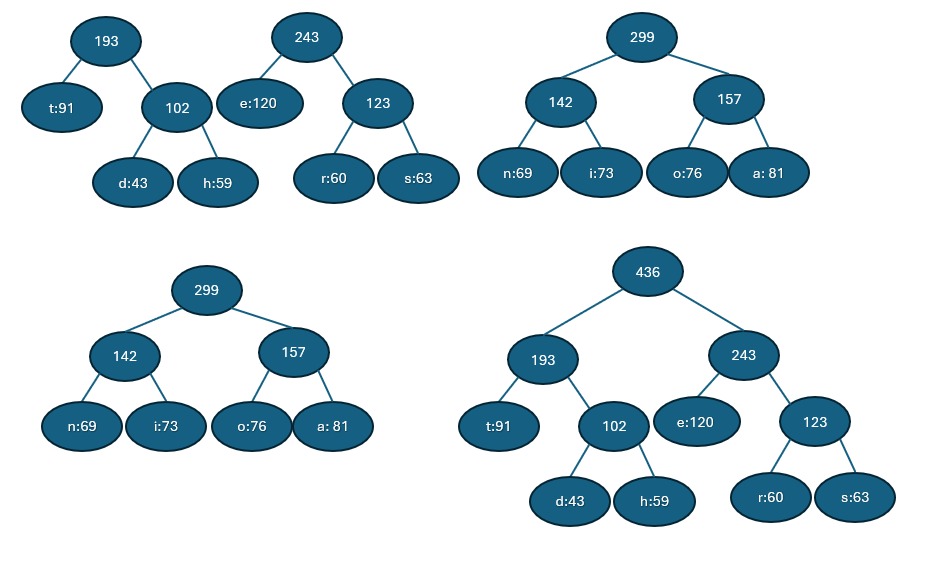
\includegraphics[width=1\textwidth]{huffman3.png}
    \subitem 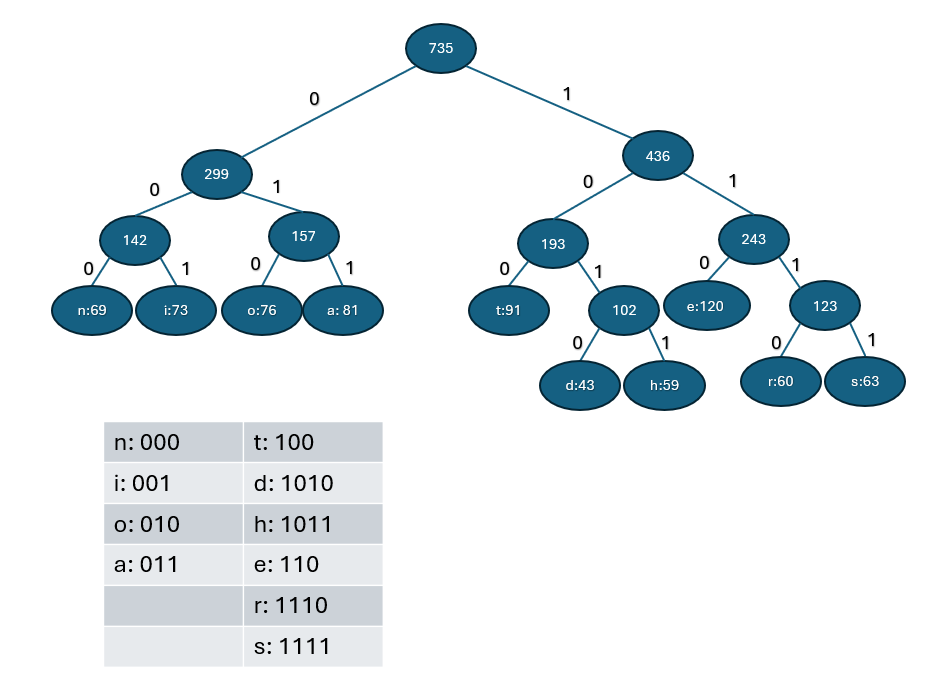
\includegraphics[width=1\textwidth]{huffman4.png}
\end{enumerate}

% Question 3
\subsection*{Q3}
\begin{enumerate}[label=(\alph*)]
    \item Find the greedy strategy for this problem:
    \subitem (1) Assumption: Each day waited, incurs a penalty $p_i$ for job $j_i$.
    \subitem (2) Assumption: Each job $j_i$ takes time $d_i$ days to complete.
    \subitem (3) Assumption: Only 1 job can be worked on at a time.
    \subitem (4) The objective function is to Minimize Total penalty: $min(\sum_{1}^{n} P_i)$
    \subitem (5) P = Total penalty incurred by each task
    \subitem (5) P = The total time used to complete previous tasks multiplied by whatever the value of $p_i$ is.
    \subitem (6) Given the objective is to minimize total penalty, we need to look for a greedy selection criteria that minimizes this penalty. To do this, I worked out a few brute force problems and decided on the following selection criteria:
    \subitem (7) Greedy Selection Criteria: $min\frac{d_i}{p_i}$
    \subitem (8) This essentially means that we are looking for the jobs with the lowest days per point of penalty. This approach will minimize the total penalty in the problem.
    
\end{enumerate}

% Question 4 (Graduate students only)
\subsection*{Q1 (Graduate students only)}
\begin{enumerate}[label=(\alph*)]
    \item This problem introduces value into the traditional "activity selector" problem. This value component requires that look at bit deeper when determining how exactly we will generate an optimal solution A. 
    \item The solution to this problem will essentially have a few moving parts, but will be similar to some of the dynamic programming work that we've done in the previous homeworks.
    \item Given: activities = $<a_1, a_2, a_3,...,a_n>$ values = $<v_1, v_2, v_3,...,v_n>$
    \item Given: start = $<s_1, s_2, s_3,...,s_n>$ finish = $<f_1, f_2, f_3,...,f_n>$
    \item The below algorithm should be able to return the highest value that is achieveable with the current set of activities. This algorithm does not currently hold any of the actual assignment data, it simply returns the highest value. To extend it to hold assignment data, I would need to have some sort of assignment matrix that tracks whether an activity is part of the current working solution of not. This algorithm works by essentially breaking the problem down into smaller subparts. So at each time step, we loop through each of the activities and determine which of them we can assign. 
    \item At each time step, we look at all tasks and determine if the value of the current task and the max value of the times before its start time, is greater than any value we've gotten before. If so, then that becomes the new max value, if not, we defer to the current max.
    \item Additional Assumptions:
    \subitem (1) We sort the list by earliest finish date
    \subitem (2) The list if sorted using an $O(nlog(n))$ algorithm
    \subitem (3) This algorithm has nested for loops that each depend on n.
    \subitem (4) Given these loops, this algorithm is $O(n^2)$
    \begin{lstlisting}[frame=single]
    def valueActivitySelector(s, f, v):
        
        times = set(s,f) // find all time indices
        currentMax = 0

        # Set max values to 0 at each time step
        for i in times:
            maxVal[i] = 0

        # Iterate through time indices
        for i in times:
            for j in range(len(s)):
                start = s[j]
                finish = f[j]
                value = v[j]

                if finish <= i:
                    maxValue = max(
                        value+maxVal[start],
                        currentMax
                        )
                    maxVal[i] = maxValue
            currentMax = maxVal[i]
        
        return currentMax
        \end{lstlisting}
\end{enumerate}


\end{document}
